\documentclass[11pt]{article}
\usepackage[english]{babel}
\usepackage[utf8x]{inputenc}
\usepackage{amsmath}
\usepackage{graphicx}
\graphicspath{{Images/}}
\usepackage{hyperref}
\usepackage{float}
\usepackage{todonotes}
\usepackage[linesnumbered,algoruled,boxed,lined]{algorithm2e}
\usepackage[a4paper, margin=2.5cm]{geometry}
\usepackage{geometry}
\usepackage[title,toc,page]{appendix}
% \usepackage{fullpage}
%\usepackage{fancyhdr}
%\pagestyle{fancy}

\begin{document}
\begin{titlepage}
\newcommand{\HRule}{\rule{\linewidth}{0.1mm}} 
\center % Center everything on the page
 
%---------------------------------------------------------------------------------
%	HEADING SECTIONS
%---------------------------------------------------------------------------------
\vfill
\textsc{\LARGE Quantum Natural Language Processing}
\vfill
%---------------------------------------------------------------------------------
%	TITLE SECTION
%---------------------------------------------------------------------------------
\HRule \\[0.4cm]
{ \Large \bfseries D1.1} \\[0.3cm]
{ \Large \bfseries Overview of DisCo Algorithms \& \\[0.1cm]Methods for Testing and Evaluation}\\[0.1cm]
\HRule \\[1.5cm]
 
%---------------------------------------------------------------------------------
%	AUTHOR SECTION 
%---------------------------------------------------------------------------------
\vfill
\begin{center} \large
\emph{Authors}\\[0.5cm]
Lee J.~\textsc{O'Riordan}, ICHEC\\[0.2cm]
Myles \textsc{Doyle}, ICHEC\\[0.2cm]
Venkatesh \textsc{Kannan}, ICHEC
\end{center}
\vfill
{\large April 15, 2019}\\[1cm] 
\vfill
\hfill
\begin{minipage}{0.4\textwidth}

\includegraphics[scale=0.3]{ichec_logo.jpeg}
\end{minipage}
\hfill
\begin{minipage}{0.4\textwidth}

\includegraphics[scale=0.3]{intel_logo.png}
\end{minipage}
\vfill

\includegraphics[scale=0.3]{ei_logo.JPG}
\vfill
\end{titlepage}

%---------------------------------------------------------------------------------
%	AUTHOR SECTION 
%---------------------------------------------------------------------------------
\section*{Executive Summary}
In Q2 2018, Intel Ireland and the Irish Centre for High-End Computing (ICHEC) identified the opportunity to leverage the Intel Quantum Simulator (qHiPSTER) to port and implement the quantum version of an existing compositional semantics NLP algorithm to analyse the meaning sentences in a given corpus. Funded by both Intel Ireland and Enterprise Ireland, this project has the following aims: (1) to leverage and evaluate the computing power that quantum devices can offer to computation intensive NLP algorithms such as in the distributional compositional semantics model; (2) to develop the ecosystem of proof-of-concept applications ported to the emerging quantum computing domain, particularly using a highly relevant application domain such as NLP; and (3) to pioneer a collaborative innovation environment in Ireland between industry and research organisations to develop expertise to program quantum computers.

In this deliverable, we report on the strategies to map an existing NLP model called DisCo (Distributional Compositional Semantics) and its component algorithms to quantum computing platforms, particularly Intel qHiPSTER. The strategies address computing and encoding the meaning spaces of a given sentence into quantum states, and computing the closeness of the meanings of two sentences. This report also presents the representative corpora and the methods that will be used to test and evaluate the implementations of the algorithms, along with an overview of the details of the Intel qHiPSTER installation on the Irish national supercomputer (Kay). We also present an overview of the open challenges that have been identified and the workarounds that are employed, along with a summary of the next steps in the project towards implementing the solution on Intel qHiPSTER.

\newpage
\tableofcontents
\newpage
\listoffigures
\listoftables

%---------------------------------------------------------------------------------
%---------------------------------------------------------------------------------
\newpage
\section{Introduction}
\label{sec:introduction}

\subsection{Abstraction of DisCo Algorithms}
\label{sec:abstraction_of_disco_algorithms}
Updates to the algorithms defined in deliverable D1.1 Section 2 ``Abstraction of DisCo Algorithms"

\subsection{Representative Corpora}
\label{sec:representative_corpora}
Recap of the representative corpa currently used for the tests and evaluation; Re-use from deliverable D1.1 if sufficient

\subsection{Structure of the Document}
The rest of the document is structured as follows: Sections \ref{sec:implementation_of_disco_algorithms} xyz; Section \ref{sec:testing_and_evaluation_of_disco_algorithms} xyz; Section \ref{sec:discussion_and_summary} summarises and discusses the next steps towards implementing the algorithms.

%---------------------------------------------------------------------------------
%---------------------------------------------------------------------------------
\newpage
\section{Abstraction of DisCo Algorithms}
\label{sec:abstraction_of_disco_algorithms}
To implement the DisCo model algorithms, we first consider the mappings between DisCo's graphical notation and quantum Dirac notation. Figure~\ref{fig:disco_dirac} represents the meaning space and mappings necessary to understand the sentence ``\textsc{Mary likes John}'', and follows directly from the work of Coecke et al. \cite{Coecke_Sadrzadeh_Clark_2010}. Above the dotted line, the blue triangles indicate each component (word) of the sentence. The lines beneath the sentence entities indicate the space in which their meanings exist; \textbf{P} and \textbf{P$^*$} indicate the meaning space of nouns and their conjugates, \textbf{S} is the overall meaning of the sentence, and verbs exist in the composite meaning space of \textsc{noun-sentence-noun}. Below the dotted line, connecting these wires allows us to perform computations on this abstract formalism, and is akin to contractions over tensor-network diagrams commonly used in condensed matter systems~\cite{ Coecke_Paquette_Pavlovic_2009,Biamonte_Clark_Jaksch_2011}. By performing these ``U''-shaped wirings, we contract these tensor indices, with the remaining free-index in the space \textbf{S} (the sentence meaning).

\begin{figure}[H]
    \centering
    \includegraphics[width=0.85\textwidth]{D1_1/Images/MappingDisCo.pdf}
    \caption{Structural mapping of DisCo graphical notation to quantum Dirac notation. }
    \label{fig:disco_dirac}
\end{figure}

This approach will require implementations of text-analysis, resource allocations, and mappings between the generated quantum states. We aim to develop a framework to ensure these mappings for sentence state-creation and meaning extraction are at high-level to enable ease of extensibility and development for more complex sentence structures. We propose the following algorithmic layout to overseeing the implementation of this work.

Algorithm~\ref{algo:tagging} is used to tokenise and tag the text in a given corpus. Using this, we can determine in which respective space a token (word) exists, as shown by the wiring in Figure~\ref{fig:disco_dirac} and create the appropriate quantum state to represent its meaning.

%%Pseudocode for corpus to tags and encodings
\begin{algorithm}\label{algo:tagging}
    \KwData{corpus strings}
    \KwResult{data encodings, tagged words, and meaning-spaces }
    load corpus strings\;
    tokenise corpus strings\;
    \While{not processed all corpus tokens}{
        read current token\;
        \uIf{token $\in~\{\,x \mid x \textrm{ is a noun}\,\}$}{
            tag token as noun\;
            }
        \uElseIf{token $\in~\{\,x \mid x \textrm{ is a verb}\,\}$}{
            tag token as verb\;
        }
        \Else{
            ignore token\;
        }
        generate unique bit-string encoding for token\;
        add tagged token to the tagged set\;
        token $\rightarrow$ next token\;
    }
    write tagged and encoded tokens to external DB\;
    \caption{Corpus to meaning-space tagging and encoding}
\end{algorithm}

\newpage
Following this step, we use Algorithm~\ref{algo:encoding} to generate the necessary quantum gate operations to encode the corpus data. This generates the quantum state with the encoded meanings, again as presented by Figure~\ref{fig:disco_dirac}. With this state, we can now examine the closest vectors and sentence similarities, through appropriately ``wiring'' test states to the resulting quantum state.

%%Pseudocode for encodings to state construction
\begin{algorithm}\label{algo:encoding}
    \KwData{tagged and encoded tokens, }
    \KwResult{quantum state representation of meaning-space }
    load tagged and encoded data, $D$\;
    initialise data quantum register, $\vert D\rangle$ to $\vert 00\cdots 0\rangle$\;
    \For{$i\leftarrow D[1]$ \KwTo $D[n]$ }{
        generate quantum gate sequence to realise $D[i]$ in quantum circuit\;
        apply gate sequence to update $\vert D\rangle$ state with $D[i]$ data\;
    }
    \caption{Corpus meaning-space quantum state creation}
\end{algorithm}

% \todo{Closest vector model}
% \todo{Sentence similarity}

Following the decomposition of a corpus using Algorithm~\ref{algo:tagging} and subsequent encoding using Algorithm~\ref{algo:encoding}, we use Algorithm~\ref{algo:closest_vector} to evaluate the closest vector for a given encoded data set with their quantum states. Algorithm~\ref{algo:closest_vector} presents a method for distance calculation between a test data vector (state) and the encoded data, and returns the representative vector (state) with closest meaning to that of the test as the output. By appropriately training the encoding data, we can affect the result, and as such different text corpora will likely produce different resulting values.

%%DisCo closest vector
\begin{algorithm}\label{algo:closest_vector}
    \KwData{quantum state representation of meaning-space $\vert \Psi \rangle$, quantum state representation of test token $\vert s \rangle$ }
    \KwResult{quantum state representation of meaning-space $\vert \Psi \rangle $ with amplitudes proportional to the distance between $\vert s \rangle $ and each state in $\vert \Psi \rangle$}
    load $\vert \Psi \rangle$ using Algorithm~\ref{algo:encoding}\;
    similarly load $ \vert s \rangle$ into separate register\;
    update amplitudes using distance calculation between $\vert s \rangle$ and each state in $\vert \Psi \rangle$;
    \caption{Closest vector problem using the DisCo framework.}
\end{algorithm}

\newpage
As a natural extension to Algorithm~\ref{algo:closest_vector}, we may encode a variety of test and data states, and determine their similarity through an inner-product evaluation, defined by Algorithm~\ref{algo:csc}.

%%DisCo sentence similarity
\begin{algorithm}\label{algo:csc}
    \KwData{quantum state data tags and tokens, \textsc{O}$_d$}
    \KwData{quantum state test tags and tokens, \textsc{O}$_t$}
    \KwResult{numerical similarity between sentences trained on corpus data}
    allocate quantum register, $\vert \Psi \rangle$ of length $2n+2$\;
    \ForEach{token $j \in \textsc{O}_d$ }{
        encode $j$ into $\vert \Psi \rangle$ using Algorithm~\ref{algo:encoding} for indices $1\rightarrow n$
    }
    \ForEach{token $k \in \textsc{O}_t$ }{
        encode $k$ into $\vert \Psi \rangle$ using Algorithm~\ref{algo:encoding} for indices $n+1\rightarrow 2n$
    }
    use Algorithm~\ref{algo:closest_vector} to compare test with encoded data\;
    return inner-product value of comparison\;
    \caption{Sentence similarity problem using the DisCo framework}
\end{algorithm}


%---------------------------------------------------------------------------------
%---------------------------------------------------------------------------------
\newpage
\section{Mapping DisCo Algorithms on Intel Quantum Simulator}
\label{sec:mapping_disco_algorithms_on_intel_quantum_simulator}
In this section, we discuss the details related to the implementation of the algorithms presented in Section~\ref{sec:abstraction_of_disco_algorithms}. The encoding of classical data into a quantum system can be achieved through a variety of means, though they can be mapped to two different approaches: state (digital) encoding, or amplitude (analogue) encoding~\cite{Schuld_2017,Mitarai_Kitagawa_Fujii_2019}. For our work on the QNLP project the use of a state encoding method for corpus representation offered the best mapping to our problem. Though, much of the problem can be described and implemented using this digital approach, the use of amplitude-based methods are well suited when results are to be obtained. We aim to operate in a mixed-mode approach: encoding and querying our data using state encoding, and obtaining the best result through amplitude modification and measurement.

The nearest-neighbour and sentence similarity algorithms rely on the encoding of a large data-set into the quantum domain, and will follow the approaches discussed in Algorithms~\ref{algo:tagging}, \ref{algo:encoding}, \ref{algo:closest_vector}, and \ref{algo:csc}. Upon these layers, we will implement quantum state engineering and control methods as discussed in the work of Zeng and Coecke~\cite{Zeng_Coecke_2016}, and supplemented by Wiebe et al.~\cite{Wiebe_Kapoor_Svore_2014} and Trugenburger~\cite{Trugenberger_2001,Trugenberger_2002}. At a high level, these methods will allow the discovery of the closest encoded vector (state) to a given test vector (state), and additionally the similarity between meanings of an encoded sentence structure, and that of a test.

%---------------------------------------------------------------------------------
%---------------------------------------------------------------------------------

% \subsubsection{Design considerations}
\subsection{Design Considerations}
\label{sec:design_considerations}
The following discussion applies to the implementation of the methods proposed in Algorithms~\ref{algo:tagging} and \ref{algo:encoding}, as well as extensions to the closest vector and sentence similarity solutions presented in Algorithms~\ref{algo:closest_vector} and \ref{algo:csc}. Figure~\ref{fig:qnlp_controlflow} illustrates the control flow of the planned implementation.

\begin{figure}[!ht]
    \centering
    \includegraphics[width=\textwidth,keepaspectratio]{D1_1/Images/QNLP_Controlflow.pdf}
    \caption{Control flow of proposed QNLP project implementation.}
    \label{fig:qnlp_controlflow}
\end{figure}

The design of this QNLP software solution is based on a two-level approach: $(i)$ the corpus analysis and formatting layer, and $(ii)$ the quantum processing layer. Layer $(i)$ will be written in Python, to avail of ease-of-use in text processing and analysis. Since this layer will be called at the initial outset of the program run, the performance impact will be negligible compared to the DisCo methods. Layer $(ii)$ will be written entirely in C++, and will directly leverage the Intel Quantum Simulator (qHiPSTER). The pre-processed data from layer $(i)$ will be loaded, and encoded into qHiPSTER to generate the full meaning-space of the analysed corpus.

%---------------------------------------------------------------------------------

\paragraph{Pre-computation:}
To analyse and prepare the corpus data for encoding into the quantum state-space, we have determined that the use of well-defined classical routines for corpus tokenisation and tagging can be achieved using the NLTK suite~\cite{BirdKleinLoper09}. Following the pre-compute step, all required data and meta-data for the qHiPSTER encoding and processing will be stored in an intermediary data format. This approach follows the methods discussed by Algorithm~\ref{algo:tagging}.

%---------------------------------------------------------------------------------

\paragraph{Alternative approach to QRAM methods:}\label{par:qram_alt_approach} The methods proposed by Zeng and and Coecke~\cite{Zeng_Coecke_2016} rely on the use of a quantum random access memory (QRAM)~\cite{Giovannetti_Lloyd_Maccone_2008} model to achieve the data access bounds proposed for the closest vector and sentence similarity problems. However, the existence and use of realisable QRAM models in quantum computing algorithms is currently assumed, yet unimplemented in practice. This is in part due to the difficulties in realising the QRAM model as originally proposed (3-level quantum states required), or the large resource requirements necessary for a qubit-implementable model~\cite{Arunachalam_Gheorghiu_Jochym-OConnor_Mosca_Srinivasan_2015}. This renders it almost unusable for real-world problems in current physical or simulated quantum computing systems with low numbers of qubits. Due to the limited number of qubits which we aim to work with, we deemed it necessary to find an alternative approach to realising the state-creation and distance methods, and subsequently Algorithms~\ref{algo:closest_vector} and \ref{algo:csc}. For the purpose of state creation, we aim to follow the approach of Trugenberger~\cite{Trugenberger_2001,Trugenberger_2002}, encoding the data by ``carving-off'' probability slices and encoding the required state information into these slices. Following this, we use an additional qubit register to store a test data vector to compare with. We make use of the Hamming distance metric between the encoded data and the test input to determine the closest encoded state.

This method allows us to avoid the use of a QRAM implementation, at the cost of an iterative state-preparation routine, as we feed in each bit-string to be encoded. The Hamming distance takes advantage of the inherent quantum parallelism offered by the register, and as such can be computed over the entire superposition state simultaneously. 

At this stage, we have several options to determine the closest vector to a known data set: follow the approaches of Trugenberger~\cite{Trugenberger_2001,Trugenberger_2002}, Schuld et al.~\cite{Schuld_Sinayskiy_Petruccione_2014}, Wiebe et al.~\cite{Wiebe_Kapoor_Svore_2014}, or follow alternative approaches defined by use of the the Durr-Hoyer (DH) algorithm~\cite{Durr_Hoyer_1996} or phase shifting. These alternative approach are discussed in further detail in Appendices~\ref{app:hamming_dh} and ~\ref{app:ry_phase}.

It may be instructive to implement many of the above mentioned approaches to determine the optimal method for the closest vector problem, using the encoding strategy and similarity calculations from \cite{Trugenberger_2001,Trugenberger_2002}, the amplitude-based approaches proposed separately by \cite{Schuld_Sinayskiy_Petruccione_2014} and \cite{Wiebe_Kapoor_Svore_2014}, as well as the modified Hamming approaches discussed above. Given any successful implementation of these methods for the closest vector problem, the extension to the sentence similarity problem is trivial. 

We can now discuss the elements of these methods as we see them mapping to our problem.

%---------------------------------------------------------------------------------
%---------------------------------------------------------------------------------

% \subsubsection{Encoding of Classical Bit Stings to Superposition of States}
\subsection{Encoding of Classical Bit Strings to Superposition of States}
\label{sec:encoding_trugenberger}
As discussed above in Section~\ref{sec:design_considerations}, the sequential methods for encoding binary strings to a superposition of states proposed by Trugenberger~\cite{Trugenberger_2001,Trugenberger_2002} will be used for encoding the binary representation of our corpus into a superposition of quantum states.

For a set of $N$ binary patterns $p^i = \{p_1^i, \dots, p_n^i \} $ for $i=1,\dots,N$ of length $n$ being encoded, we can encode these patterns into a quantum superposition of states such that

\begin{align}
    \label{eqn:superposition_state}
    \vert m \rangle = \frac{1}{\sqrt{N}}\sum\limits_{i=1}^ {N} \vert p^i \rangle.
\end{align}

Trugenberger developed a sequential method for creating the superposition $\vert m \rangle$ in \cite{Trugenberger_2001}, by first loading a pattern into an auxiliary register, which was then copied into $\vert m \rangle$, the memory qubit register. This process being repeated for each binary pattern to encode, ``carving'' off the newly encoded state term from the already encoded terms while maintaining the appropriate normalization factors in the amplitudes. This method required $2n + 2$ qubits. It will be referred to as method $1$. 

Trugenberger generalizes this method in \cite{Trugenberger_2002} which generates the superposition of states $\vert m \rangle$, by applying a unitary matrix to the state $\vert 0_1\dots 0_n \rangle$. The process is repeated for each input binary pattern using the aforementioned ``carving'' off method to store the new term in a state. This method requires only $n+2$ qubits, which is a significant reduction from method 1. This will be referred to as method $2$.

The main idea of both methods is detailed below:\\

\noindent
\begin{minipage}[b]{0.45\textwidth}
\textbf{Method 1:}
\begin{align*}{}
\vert \psi_0 \rangle & =  \vert p_1^1,\dots,p_n^1\rangle\vert 01\rangle\vert0_1,\dots,0_n \rangle\\
\vert \psi_1 \rangle & =  \prod\limits_{j=1}^{n} \textrm{2XOR}_{p_j^i u_2 m_j} \vert \psi_0 \rangle\\
\vert \psi_2 \rangle & =  \prod\limits_{j=1}^{n} \textrm{NOT}_{m_j} \textrm{XOR}_{p_j^i m_j}  \vert \psi_1 \rangle\\
\vert \psi_3 \rangle & =  \textrm{nXOR}_{m_1\dots m_n u_1}  \vert \psi_2 \rangle\\
\vert \psi_4 \rangle & =  \textrm{CS}_{u_1 u_2}^{p+1-i}  \vert \psi_3 \rangle\\
\vert \psi_5 \rangle & =  \textrm{nXOR}_{m_1\dots m_n u_1}  \vert \psi_4 \rangle\\
\vert \psi_6 \rangle & =  \prod\limits_{j=n}^{1} \textrm{XOR}_{p_j^i m_j} \textrm{NOT}_{m_j}  \vert \psi_5 \rangle\\
\vert \psi_7 \rangle & =  \prod\limits_{j=n}^{1} 2\textrm{XOR}_{p_j^i u_2 m_j} \vert \psi_6 \rangle
\end{align*}
\hspace{10pt}\\
\hspace{10pt}
\end{minipage}
\begin{minipage}[b]{0.45\textwidth}
\textbf{Method 2:}
Let us define the single qubit unitary gate
\begin{align*}{}
U_j^i = \cos\left(\frac{\pi}{2} p_j^i\right)1 + \sin \left(\frac{\pi}{2} p_j^i\right)\sigma_y.
\end{align*}
For a pattern $p^i$, we can encode the pattern into a single state by applying $U_j^i$;
\begin{align*}
    \vert p^i \rangle = \prod\limits_{j=1}^n U_j^i \vert 0_1\dots 0_n\rangle.
\end{align*}

Then to store it in a superposition state given initial state $\vert\psi_0\rangle$, we compute the following;
\begin{multline*}
    \vert\psi_0 \rangle = \vert 0_1\dots0_n\rangle\vert00\rangle\\
    \vert\psi_1 \rangle = \prod\limits_{j=1}^{n} \left[\left( \textrm{CP}_{u_2}^{i}\right)^{-1} \textrm{NOT}_{u_1} \textrm{CS}_{u_1u_2}^{p+1-i} \textrm{XOR}_{u_{2}u_{1}} \textrm{CP}_{u_{2}}^{i}\right] \\ \times \textrm{NOT}_{u_2} \vert\psi_0\rangle.   
\end{multline*}
\end{minipage}

Repeating either process appropriately for different inputted binary patterns allows us to build an encoded data superposition state in a reliable manner.

It is observed that method $2$ is more efficient than method 1 in terms of the number of qubits required. Method $2$ also requires less operations than method $1$, hence is less computationally expensive. Therefore, method $2$ appears to be the best approach out of the two to use as an encoding strategy. For the sake of completeness and for comparison, both methods will be implemented.

Both of the aforementioned methods are realizable using the Intel Quantum Simulator since they use well defined quantum gate operations including the NOT, XOR, 2XOR (Toffoli) and CU (controlled unitary) gates. We have also developed some necessary extensions of the standard routines available in Intel's Quantum Simulator, including the $n$-qubit controlled unitary gate (nCU), which is required in the form of an n-qubit controlled not (nCX) gate for method 1. Hence, both methods prove to be reliable approaches to proceed with. To implement either method, the following unitary matrix must be first constructed for $i = 1,\dots,N$.
\begin{align*}
    S^i = 
    \begin{bmatrix}
        \sqrt{\frac{i-1}{i}} & \frac{1}{\sqrt{i}} \\
        -\frac{1}{\sqrt{i}}  & \sqrt{\frac{i-1}{i}}
    \end{bmatrix},
\end{align*}
$S^i$ is applied using the controlled unitary operator with $S^i$ being the corresponding unitary matrix. The quantum operations required to implement both methods are displayed above. Each operation used is directly implementable using the Intel Quantum Simulator, apart from nXOR which required an extension of the available gate operations.

%---------------------------------------------------------------------------------
%---------------------------------------------------------------------------------

% \subsubsection{Hamming Distance}\label{sub:hamming_dist}
\subsection{Hamming Distance for Sentence Similarity}\label{sub:hamming_dist}
Two approaches to calculate the Hamming distance are proposed. One, being Trugenberger's, the other a variation of Trugenberger's Hamming distance subroutine developed by Schuld et al.~\cite{Trugenberger_2001, Schuld_Sinayskiy_Petruccione_2014}. For a known test word represented as a binary state, we can calculate the Hamming distance between this word's representation and every other basis word in the superposition. The approach pulls the Hamming distance into the eigenvalue of the eigenstate corresponding to each individual term in the superposition. Thus, the Hamming distance can be stored in the amplitude of its corresponding state. This enables us to quantify the similarity in meaning between the test word and the set of basis words, resulting in the test word's meaning.

The algorithm is detailed in Dirac notation as defined by Trugenberger \cite{Trugenberger_2001} as follows. Given the superposition of encoded binary patterns $\vert m \rangle$ as defined in Eq.~\eqref{eqn:superposition_state} which will be denoted as register $m$, we define two extra registers $d$ of length $n$ and $c$ of length $1$. Thus a total of $2n + 1$ qubits are required for this stage of the calculation. Note, that the auxiliary register of the previous encoding strategy can be reused here, reducing the overhead of the number of qubits used. We define our initial state to be the tensor product of these three registers, where $c$ is in the state $\vert 0 \rangle$ and the register $d$ is the binary test pattern $x = x_1,\dots,x_n$. Thus,

\begin{align*}
    \vert \psi_0 \rangle &= \frac{1}{\sqrt{N}}\sum\limits_{i=1}^{N} \vert x \rangle \vert p^i \rangle \vert 0 \rangle \\
    &= \frac{1}{\sqrt{N}}\sum\limits_{i=1}^{N} \vert x_1\dots x_n\rangle\vert p_{1}^{i}\dots p_{n}^{i}\rangle \vert 0 \rangle
\end{align*}

The next step is to apply a Hadamard operation to the auxiliary qubit;
\begin{align*}
    \vert \psi_1 \rangle = \frac{1}{\sqrt{2N}}\sum\limits_{i=1}^{N} \vert x_1\dots x_n\rangle\vert p_{1}^{i}\dots p_{n}^{i}\rangle \vert 0 \rangle + \frac{1}{\sqrt{2N}}\sum\limits_{i=1}^{N} \vert x_1\dots x_n\rangle\vert p_{1}^{i}\dots p_{n}^{i}\rangle \vert 1 \rangle
\end{align*}

The Hamming distance between $x$ and $p^i$ for $j=1,\dots, n$ is then calculated in binary format and stored in the $d$ register overwriting the test pattern stored there. This is done by flipping all qubits in register $d$, then applying a controlled-NOT gate on each qubit in register $d$ with the corresponding qubit in $m$ acting as control;

\begin{align*}
    \vert \psi_2 \rangle &= \prod\limits_{j=1}^{n}\textrm{X}_{x_j} \textrm{CNOT}_{x_{j}p_{j}^{i}} \vert \psi_1 \rangle\\
    &= \frac{1}{\sqrt{2N}}\sum\limits_{i=1}^{N} \vert d_1^i\dots d_n^i\rangle\vert p_{1}^{i}\dots p_{n}^{i}\rangle \vert 0 \rangle + \frac{1}{\sqrt{2N}}\sum\limits_{i=1}^{N} \vert d_1^i\dots d_n^i\rangle\vert p_{1}^{i}\dots p_{n}^{i}\rangle \vert 1 \rangle
\end{align*}

\noindent where $d_j^i$ is the distance between the test pattern and the $i^{\textrm{th}}$ training pattern for their $j^{\textrm{th}}$ qubit. Due to a technique used later in the algorithm, it is desired that similar patterns will have a large Hamming distance, hence we say

\begin{align*}
    d_j^i =
    \begin{cases}
        1 \quad \textrm{if } \vert v_j^i \rangle = \vert p_j^i \rangle,\\
        0 \quad \textrm{otherwise}
    \end{cases}
\end{align*}

\noindent which is why the \textrm{NOT} gate was applied to the $m$ register.

The next step is to pull the Hamming distance into the amplitude of its corresponding state. This is done by applying the Hamiltonian

\begin{align*}
    \mathcal{H} = \sum\limits_{j=1}^{n}\left(\frac{\sigma_z + 1}{2}\right)_{d_j} \otimes 1 \otimes \left(\sigma_z\right),
\end{align*}

\noindent through the unitary operator 
\begin{align*}
    U = e^{-\imath \frac{\pi}{2n}\mathcal{H}}.
\end{align*}

Thus we obtain the state

\begin{align*}
    \vert \psi_3 \rangle &= e^{-\imath \frac{\pi}{2n}\mathcal{H}} \vert \psi_2 \rangle \\
    &= \frac{1}{\sqrt{2N}}\sum\limits_{i=1}^{N} e^{\imath \frac{\pi}{2n}d_\mathcal{H}\left(\Vec{x},\vec{p^i}\right)} \vert d_1^i\dots d_n^i\rangle\vert p_{1}^{i}\dots p_{n}^{i}\rangle \vert 0 \rangle + \frac{1}{\sqrt{2N}}\sum\limits_{i=1}^{N} e^{-\imath \frac{\pi}{2n}d_\mathcal{H}\left(\Vec{x},\Vec{p^i}\right)} \vert d_1^i\dots d_n^i\rangle\vert p_{1}^{i}\dots p_{n}^{i}\rangle \vert 1 \rangle,
\end{align*}

\noindent where $d_\mathcal{H}\left(\Vec{x},\Vec{p^i}\right)$ is the Hamming distance between $\Vec{x}$ and $\Vec{p^i}$ with the closer the value is to $n$, the more similar the patterns are to each other.

Finally, applying a Hadamard to the control register $c$, the new state reduces to

\begin{align*}
    \vert \psi_4 \rangle = \frac{1}{\sqrt{2N}}\sum\limits_{i=1}^{N} \cos\left[ \frac{\pi}{n}d_\mathcal{H}\left(\Vec{x},\vec{p^i}\right) \right] \vert d_1^i\dots d_n^i\rangle\vert p_{1}^{i}\dots p_{n}^{i}\rangle \vert 0 \rangle \\ + \frac{1}{\sqrt{2N}}\sum\limits_{i=1}^{N} \sin\left[ \frac{\pi}{n}d_\mathcal{H}\left(\Vec{x},\Vec{p^i}\right)\right] \vert d_1^i\dots d_n^i\rangle\vert p_{1}^{i}\dots p_{n}^{i}\rangle \vert 1 \rangle.
\end{align*}

Due to the nature of measurement of a quantum system it is not possible to obtain the amplitude of each state directly. Instead, we can obtain the probability of each quantum state (training pattern) occurring $\mathcal{P}\left( p^i\right)$. This probability is influenced by the Hamming distance in such a way that higher probabilities correspond to a higher Hamming distance, indicating that the test pattern is close to that particular training pattern.

To conduct this measurement, we must first collapse the auxiliary cubit in register $c$. If it collapses to $\vert0\rangle$ with a high probability, then the test pattern is very different from all of the training patterns. Otherwise, if it collapses to $\vert 0 \rangle$ with a high probability, then the test pattern is close to the training patterns. More formally,

\begin{align*}
    \mathcal{P}\left(\vert c \rangle = \vert 0 \rangle \right) &= \frac{1}{N} \sum\limits_{i = 1}^{N} \cos^2 \left[\frac{\pi}{2n} d_\mathcal{H}\left(\Vec{x},\vec{p^i}\right)\right], \\
    \mathcal{P}\left(\vert c \rangle = \vert 1 \rangle \right) &= \frac{1}{N} \sum\limits_{i = 1}^{N} \sin^2 \left[\frac{\pi}{2n} d_\mathcal{H}\left(\Vec{x},\vec{p^i}\right)\right].
\end{align*}

The probability of each individual pattern occurring can be obtained by repeating the experiment for a large number of times, measuring the register $m$ corresponding to the training pattern, and recording the observed state of this register. Thus a distribution of probabilities of each state occurring can be obtained. Furthermore, we know that 

\begin{align*}
    \mathcal{P}\left(\vert m \rangle = \vert p^i \rangle \right) = \frac{1}{N\mathcal{P}\left(\vert c \rangle = \vert 0 \rangle \right)} \cos^2 \left[\frac{\pi}{2n} d_\mathcal{H}\left(\Vec{x},\vec{p^i}\right)\right],    
\end{align*}

\noindent and so the Hamming distance can be obtained. Note that the slightly different method used by Schuld et al. \cite{Schuld_Sinayskiy_Petruccione_2014} associates each training pattern with a class which is also encoded into the superposition. Measurement is then conducted on the class qubits rather than the training pattern qubits. These methods will also be considered as trivial extensions to Trugenberger's method.

It is also worth noting that Trugenberger proposed a version of the Hamming distance memory retrieval algorithm which uses only a unitary operator to fuse the standard quantum gate operations in a similar way as discussed in method $1$ of Section \ref{sec:encoding_trugenberger}. This method, or a slight modification of it, will also be examined to determine on which performs best.  

%---------------------------------------------------------------------------------
%---------------------------------------------------------------------------------

\iftrue
%\iffalse
\paragraph{Hamming distance similarity example:}\label{par:example_hamming}
The method introduced here demonstrates the use of the Hamming distance as discussed earlier in Section~\ref{sub:hamming_dist}, to outline a sample closest vector (state) problem.
We define a set of orthogonal words (i.e. words with no overlapping meaning) through which we can define the meaning of other words. For this test case, we choose a simple vocabulary. Following the work of Coecke et al., we opt for the simplified \textsc{noun-verb-noun} sentence structure, and define sets of words within each of these spaces, through which we can construct our full meaning space. For nouns, we have two sets, $n_s = \{\textsc{adult},\textsc{child},\textsc{smith},\textsc{surgeon}\}$ and $n_o = \{\textsc{outside},\textsc{inside}\}$, and for verbs, $v = \{\textsc{stand},\textsc{sit},\textsc{move},\textsc{sleep}\}$. With this \textsc{noun-verb-noun} meaning space sentence structure, we can calculate this as

\begin{equation*}
\left(
\begin{array}{c}
\textsc{adult} \\\\
\textsc{child} \\\\
\textsc{smith} \\\\
\textsc{surgeon} \\\\
\end{array}
\right) \otimes
\left(
\begin{array}{c}
\textsc{stand} \\\\
\textsc{sit} \\\\
\textsc{move} \\\\
\textsc{sleep} \\\\
\end{array}
\right) \otimes
\left(
\begin{array}{c}
\textsc{outside} \\\\
\textsc{inside} \\\\
\end{array}
\right)
\end{equation*}

For the above meaning-space, we can begin to define entities that exist in this space, and choose to encode them into quantum states as follows:
\begin{itemize}
    \item $\textsc{John is an adult, and a smith}$. The state is defined as \\ $\vert \textsc{John} \rangle = 1/\sqrt{2}\left(\vert \textsc{adult} \rangle + \vert \textsc{smith} \rangle\right)$, which is a superposition of the number of matched entities from the basis set.
    \item $\textsc{Mary is a child, and a surgeon}$. The state is defined as \\ $\vert \textsc{Mary} \rangle = 1/\sqrt{2}\left(\vert \textsc{child} \rangle + \vert \textsc{surgeon} \rangle\right)$, again, following the same procedure as above.
\end{itemize}

\noindent With these definitions, we can look at some sentences with \textsc{John} and \textsc{Mary}. An example corpus with meaning that can exist in our meaning-space is:
\textsc{John rests outside, and Mary walks inside}.

In this instance, we also require meanings for \textsc{rests} and \textsc{walks}. If we examine synonyms for \textsc{rests} and cross-compare with our chosen vocabulary, we can find \textsc{sit} and \textsc{sleep}. Similarly, for \textsc{walks} we can have \textsc{stand} and \textsc{move}. We can define the states of these words as $\vert \textsc{rest} \rangle = 1/\sqrt{2}\left(\vert \textsc{sit} \rangle + \vert \textsc{sleep} \rangle\right)$ and $\vert \textsc{walk} \rangle = 1/\sqrt{2}\left(\vert \textsc{stand} \rangle + \vert \textsc{move} \rangle\right)$.
Now that we have a means to define the states in terms of our vocabulary, we can begin constructing quantum states to encode the data: firstly, however, we must decide on how to encode the states.

We can give each entity in the sets of nouns and verbs a unique binary index, where the word can be mapped to the binary string (gives the encoding value), and inversely mapped back (decoding value). Classically, we can use a key-value pair for this task, wherein the key (word) gives the value (index), and vice versa. As we intend to encode this data into quantum states, we opt for a sufficient number of qubits to define our states: namely, we require $\lceil \log_2({\textrm{num elements})} \rceil$ qubits to represent our data from each respective set.

For this example, we opt for the following mappings:

\begin{equation*}
\begin{array}{c|c|c}
\mathbf{Dataset} & \mathbf{Word} & \mathbf{Bin.~Index} \\
\hline
{n_s} & \textsc{adult} & 00 \\
{n_s} & \textsc{child} & 01 \\
{n_s} & \textsc{smith} & 10 \\
{n_s} & \textsc{surgeon} & 11 \\
\\
{v} & \textsc{stand} & 00 \\
{v} & \textsc{move} & 01 \\
{v} & \textsc{sit} & 10 \\
{v} & \textsc{sleep} & 11 \\
\\
{n_o} & \textsc{inside} & 0 \\
{n_o} & \textsc{outside} & 1 \\
\end{array}
\end{equation*}

It should be noted that here we have chosen a na\"ive mapping for our key-value pairs; the use of a Gray code~\cite{gray_code}, or alternative encoding strategies, may provide more instructive meanings to the meaning-space queries later. However, we leave this to future work for implementation and testing, and use the proposed encoding method for this example.
To encode the meaning of the statement \textsc{John rests outside, and Mary walks inside}, we define the following quantum states:

\begin{equation*}
\begin{array}{c|c|c}
\mathbf{Dataset} & \mathbf{Word} & \mathbf{State} \\
\hline
{n_s} & \textsc{John} & (\vert 00 \rangle + \vert 10 \rangle)/\sqrt{2} \\
{n_s} & \textsc{Mary} & (\vert 01 \rangle + \vert 11 \rangle)/\sqrt{2} \\
{v} & \textsc{walk} & (\vert 00 \rangle + \vert 01 \rangle)/\sqrt{2} \\
{v} & \textsc{rest} & (\vert 10 \rangle + \vert 11 \rangle)/\sqrt{2} \\
{n_o} & \textsc{inside} & \vert 0 \rangle  \\
{n_o} & \textsc{outside} & \vert 1 \rangle  \\
\end{array}
\end{equation*}

We construct our quantum state by tensoring these entities, following the \textsc{noun-verb-noun} DisCo-like formalism. If we consider the \textsc{John} and \textsc{Mary} sentences separately for the moment, they are respectively given by the states $(1/2)*(\vert 00 \rangle + \vert 10 \rangle)\otimes (\vert 10 \rangle + \vert 11 \rangle)\otimes \vert 0 \rangle$ for John, and $(1/2)*(\vert 01 \rangle + \vert 11 \rangle)\otimes (\vert 00 \rangle + \vert 01 \rangle)\otimes \vert 1 \rangle$ for Mary. Tidying these up and multiplying out gives 

\begin{equation*}
\begin{array}{ccc}
\textsc{John rests outside} & \rightarrow & \frac{1}{2}(\vert 00100 \rangle + \vert 00110 \rangle +\vert 10100 \rangle +\vert 10110 \rangle) \rightarrow \vert J\rangle, \\
\\
\textsc{Mary walks inside} & \rightarrow & \frac{1}{2}(\vert 01001 \rangle + \vert 01011 \rangle +\vert 11001 \rangle +\vert 11011 \rangle) \rightarrow \vert M\rangle,\\
\end{array}
\end{equation*}
where the full meaning is given by $\vert S\rangle = \frac{\vert J \rangle + \vert M \rangle}{\sqrt{2}}$, which is a superposition of the 8 unique encodings defined by our meaning-space and sentence. 

From here, we can now introduce an additional register of equal size to $\vert S\rangle$, wherein we will encode a test vector for comparison against the encoded meanings, denoted as $\vert T \rangle$. This test vector will be overwritten with the Hamming distance of it against the other states, with the resulting value giving the intended meaning, or closest possible meaning to that of the test. Continuing with our example, we use ``Adults stand inside'', which is encoded as $\vert T \rangle = \vert 00000 \rangle$. Constructing our query state, $\vert Q \rangle = \vert T \rangle \otimes \vert S\rangle$, we get the following fully expanded state

\begin{eqnarray*}
\vert Q \rangle = \frac{1}{2/\sqrt{2}} (\vert 00000 \rangle\vert 00100 \rangle + \vert 00000 \rangle\vert 00110 \rangle + \vert 00000 \rangle\vert 10100 \rangle + \vert 00000 \rangle\vert 10110 \rangle \\+\vert 00000 \rangle\vert 01001 \rangle + \vert 00000 \rangle\vert 01011 \rangle + \vert 00000 \rangle\vert 11001 \rangle + \vert 00000 \rangle\vert 11011 \rangle).
\end{eqnarray*}
Marking the Hamming distance between both registers, and overwriting the test register modifies the above state to
\begin{eqnarray*}
\vert Q^{\prime} \rangle = \frac{1}{2/\sqrt{2}} (\vert 00100 \rangle\vert 00100 \rangle + \vert 00110 \rangle\vert 00110 \rangle + \vert 10100 \rangle\vert 10100 \rangle +  \vert 10110 \rangle\vert 10110 \rangle \\+\vert 01001 \rangle\vert 01001 \rangle + \vert 01011 \rangle\vert 01011 \rangle + \vert 11001 \rangle\vert 11001 \rangle + \vert 11011 \rangle\vert 11011 \rangle).
\end{eqnarray*}

This example is simple as any state differing from $\vert 00\cdots\rangle$ flips the test when a $\vert 1\rangle$ is seen in the training. The data in register $\vert T \rangle$ now encodes the number of different flips between both test and training data; thus, it can be seen as a similarity measure, and the state with the fewest flips will give the closest meaning to the posed test. The above example has only a single data set with one flip, that of $\vert 00100 \rangle$. By decoding the result using the mapping provided earlier, we can see that this corresponds with a meaning of \textsc{Adult(s) sit inside}. We can subsequently see that this data will give a non-zero overlap with $\vert J \rangle$.

The above approach can be mapped directly onto a qubit register, with indices used for partitioning into sub-registers. As such, the above methods can be directly implemented on qHiPSTER.

%There are some remaining questions on implementing this, however. Firstly, ensuring that the Hamming distance is encoded correctly, and such that the amplitudes are adjusted to respect the minimal difference has the highest probability of outcome. Additionally, if we wish to compare that statement with the previous corpus, we need to determine which statement encoded the resulting data-set --- a problem unless we aim to calculate many overlap integrals.

\fi
%---------------------------------------------------------------------------------
%---------------------------------------------------------------------------------


%---------------------------------------------------------------------------------
%---------------------------------------------------------------------------------
\newpage
\section{Representative Corpora}
\label{sec:representative_corpora}
For the purposes of our implementation, we have opted for some simple corpora examples. Given the ambiguity and complexity of many natural languages, we have decided to maintain a simple data set for use during our development stages.

To follow the DisCo model as proposed, we opt for the commonly discussed sentence structure of \textsc{noun-verb-noun}~\cite{Zeng_Coecke_2016,Coecke_Sadrzadeh_Clark_2010} for the majority of our development and testing. We choose a small sample of public domain and custom phrases to analyse for this type of sentence structure in increasing levels of difficulty:
\begin{itemize}
    \item User-defined simple \textsc{noun-verb-noun} statements (e.g. ``Mary likes fish, John likes cake''). Follows the example presented in Section~\ref{par:example_hamming}.
    \item Jack and Jill (nursery rhyme). Largely follows simple structure, though more complex structure than previous example.
    \item Peter Pan (Page 1, paragraph 1). Most complex example. Large departure from \textsc{noun-verb-noun} style.
\end{itemize}
For the early stages of implementation and development the above listed text corpora should suffice to allow us methods to evaluate the QNLP functionality and performance. While we expect longer corpora to be used later in the project, we currently think it best to choose those at a later date based on some realistic test cases involving the implemented methods. While a general purpose solution would be ideal, it may be required to adapt the longer corpora based on criteria we later determine from the implementations themselves.


%---------------------------------------------------------------------------------
%---------------------------------------------------------------------------------


%---------------------------------------------------------------------------------
%---------------------------------------------------------------------------------
\newpage
\section{Testing and Evaluation Methodologies}
\label{sec:testing_and_evaluation_methodologies}

\subsection{Proposed Methods for Testing}
\label{sec:proposed_methods_for_testing}

\subsubsection{Unit}\label{ss:unit}
For each individual software component (class, method, etc.) developed in the project, an associated unit-test will be deployed to verify its correctness. The Catch2 testing framework~\cite{catch2} appears to be an ideal means to allow this, with header-only requirements on the C++ layer, and is available under the Boost Software License.
%---------------------------------------------------------------------------------

\subsubsection{Integration}\label{ss:integration}
Like unit testing, we can again rely on the Catch2 framework to implement integration tests using a well-defined set of examples for each component of the Intel-QNLP suite. The use of continuous integration (CI) framework can be used to routinely examine these tests.

%---------------------------------------------------------------------------------

\subsubsection{Regression}\label{ss:regression}
As with Section~\ref{ss:integration}, we can use CI frameworks to perform periodic tests of those outlined for the previous levels of granularity in Unit and Integration tests, but also consider additional metrics such as:
\begin{itemize}
    \item Vectorisation and threading
    \item Strong and weak scaling
    \item Memory occupancy
    \item Compute and memory intensity using roofline models
    \item MPI load-balancing
    \item Additional compilation options (inter-procedural/link-time optimisation, compiler optimisation levels, fast-math, etc.) 
\end{itemize}

%---------------------------------------------------------------------------------

\subsection{Proposed Methods for Evaluation}
\label{sec:proposed_methods_for_evaluation}

\subsubsection{Acceptance}\label{ss:acceptance}
This final level of testing and evaluation will be used to determine overall correctness of the routines with a set of well-known results for the suite. We can use a manually-defined model, and compare the results to the computed data in an automated manner, making use of the CI testing methods as proposed by the Section~\ref{ss:integration}. Additionally, we may use classical NLP methods to compare results with the implemented DisCo model, such as discussed below.

%---------------------------------------------------------------------------------

\paragraph{spaCy:}
spaCy~\cite{spacy2} provides an industry-backed framework for natural language processing, which includes semantic comparison, and diagrammatic dependency visualisation. For the diagrammatic structure proposed by Zeng et al.~\cite[Example 5.3]{Zeng_Coecke_2016}, the authors derive a graph for computing the meaning of a sentence using the proposed DisCo framework. While subtle differences exist, a similar graphical style can be obtained through use of the spaCy \textit{displaCy} module. Figure \ref{fig:spacy_vs_disco} shows a comparison between both formats, wherein $(a)$ is derived manually using the model proposed by Zeng et al., and $(b)$ can be automatically derived using spaCy, both defined for the sentence ``\textit{John saw Mary read a book.}''. This provides us with a promising candidate for comparative analysis of structure for our proposed model and implementation. Additionally, spaCy provides semantic similarity comparison based on use of word-vectors, provides us with a direct means to evaluate sentence similarity using classical NLP methods. 

%---------------------------------------------------------------------------------

\paragraph{SEMILAR:}
SEMILAR~\cite{semilar_2013} is a Java tool-kit for performing semantic sentence similarity analysis on text corpora. We have not currently investigated its use for this task, but leave it as a potential means to generate comparative data as a future task.

\begin{figure}[H]
    \centering
    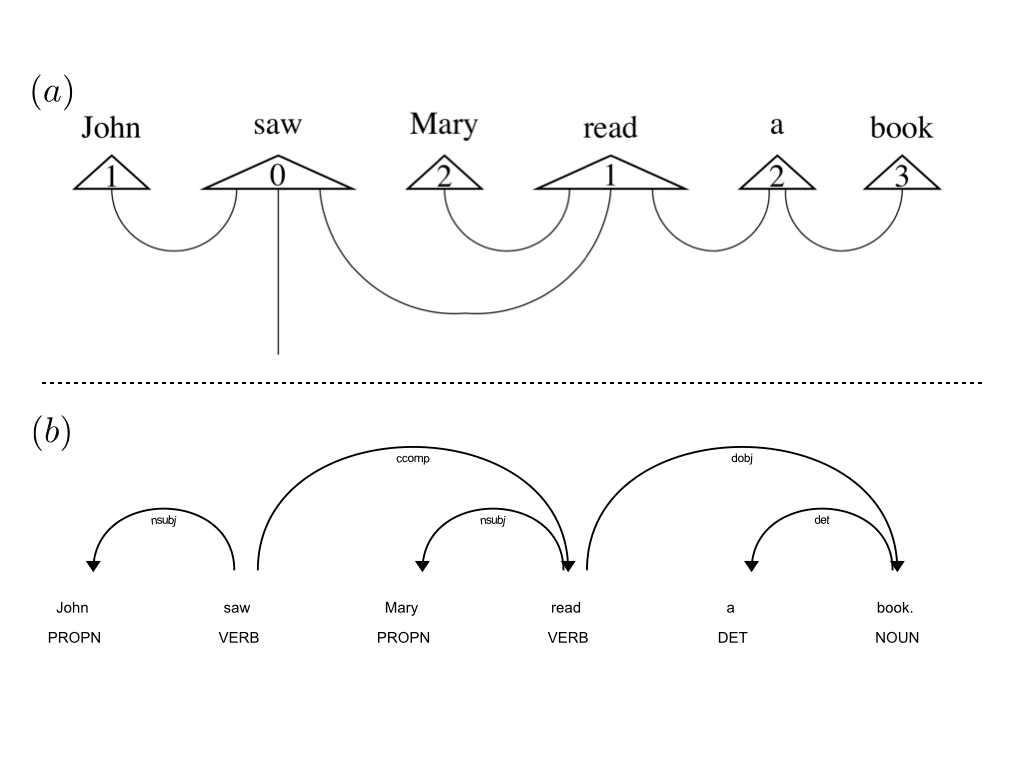
\includegraphics[width=0.85\linewidth,trim=0 20px 0 20px]{D1_1/Images/spacy_vs_CSC.png}
    \caption[DisCo model versus spaCy sentence analysis.]{Sentence parsing structure for $(a)$ the DisCo model, and $(b)$ that from the classical NLP package spaCy.}
    \label{fig:spacy_vs_disco}
\end{figure}

%---------------------------------------------------------------------------------


%---------------------------------------------------------------------------------
%---------------------------------------------------------------------------------
\newpage
\section{Intel Quantum Simulator on Kay}
\label{sec:intel_quantum_simulator_on_kay}

%---------------------------------------------------------------------------------
\subsection{Installation Setup}
\label{sec:installation_setup}
The Irish national supercomputer (Kay) was installed in August 2018, is operated by ICHEC and is comprised of
\begin{itemize}
    \item a 336 node cluster.
    \item 13,440 CPU cores, 63 TB distributed memory.
    \item Dual-socket 20-core Intel Xeon Gold (Skylake) 6148 at 2.4 GHz with 192 GB memory.
    \item 400 GB local SSD scratch.
    \item 100 GB Intel OmniPath network.
    \item Additional partitions
    \begin{itemize}
        \item Intel Xeon Phi (Knights Landing architecture).
        \item High-memory 1.5 TB RAM with 1TB local SSD scratch.
        \item Dual NVIDIA Tesla V100.
    \end{itemize}
\end{itemize}

The \textit{master} branch of the Intel Quantum Simulator from the \href{https://github.com/intel/Intel-QS/tree/master}{intel/Intel-QS} GitHub repository was installed on Kay in the path \texttt{/ichec/work/ichec001/}. The simulator was built with Intel Parallel Studio XE 2018 update 4 and vectorisation was enabled using AVX512 instead of the default SSE2.

%---------------------------------------------------------------------------------
\subsection{Performance and Scaling}
\label{sec:performance_and_scaling}
Testing was conducted using the \textit{tests/qft\_test.cpp} application supplied with the simulator which conducted a quantum Fourier transform using a specified number of qubits. Experiments were conducted for this application to demonstrate its weak and strong scaling performance. Due to the large memory footprint of the number of states, which doubles as the number of qubits increases by one, and the overhead of the corresponding access of that memory, the application was expected to be memory bound, and thus have relatively good weak scaling performance. As the number of quantum gate operations is increased in a quantum circuit the number of classical gates required to conduct the simulation can increase very quickly since these quantum gates are applied to an increasing number of qubits. Therefore, as the number of qubits are increased, the number of classical operations would increase significantly. Thus applications on the Intel Quantum Simulator are also subject to being compute bound.

Table \ref{tab:scaling_experiment_config} details the configuration of each experiment for both strong and weak scaling using double and also single precision numbers to represent the states. Figure~\ref{fig:strong_scaling} illustrates the results of the strong scaling performance and Figure~\ref{fig:weak_scaling} that of the weak scaling experiments.
Both Figure~\ref{fig:strong_scaling} and Figure~\ref{fig:weak_scaling} appear to scale approximately in a linear fashion. This implies that the application scaled relatively well for both weak and strong scaling. However, it would be desirable to conduct more experiments for larger problem sizes to further observe the scalability of the application. This was not possible due to the previously mentioned limit of the MPI message size.
% It must also be noted that the double precision performance for weak scaling was notably worse than that of single precision. However, it appears to perform worse by approximately the addition of a constant, which does not prove to be a significant issue.

\begin{table}[H]
\centering
    \begin{tabular}{|c|c|c||c|c||c|c|}
        \hline
        \multicolumn{3}{|c||}{Scaling} & \multicolumn{2}{|c||}{Strong} & \multicolumn{2}{|c|}{Weak}\\
        \hline
        Nodes           &  p    & NumProcs   & Local States  & Qubits      & Local States & Qubits \\
                   &     &  $2^p$  &  $ 2^{n-p}$  &   $n$      & $ 2^{n-p} = 2^{27}$ &  $n$\\
    
        \hline
        1               &   1   & 2                     & $2^{28-1}$                        & 28         &$2^{28-1}$&  28\\
        2               &   2   & 4                     & $2^{28-2}$                         & 28        &$2^{29-2}$&  29 \\
        4               &   3   & 8                     & $2^{28-3}$                         & 28        &$2^{30-3}$&  30 \\
        8               &   4   & 16                    & $2^{28-4}$                         & 28        &$2^{31-4}$&  31 \\
        16              &   5   & 32                    & $2^{28-5}$                         & 28        &$2^{32-5}$&  32 \\
        32              &   6   & 64                    & $2^{28-6}$                         & 28        &$2^{33-6}$&  33 \\
        64              &   7   & 128                   & $2^{28-7}$                        & 28         & $2^{34-7}$& 34 \\
     \hline
    \end{tabular}
    \caption{Details of number of total qubits, and local number of states per process for the corresponding experiment for both strong and weak scaling. }
    \label{tab:scaling_experiment_config}
\end{table}

\begin{figure}[H]
	\centering
	\begin{minipage}{.5\linewidth}
		\centering
		%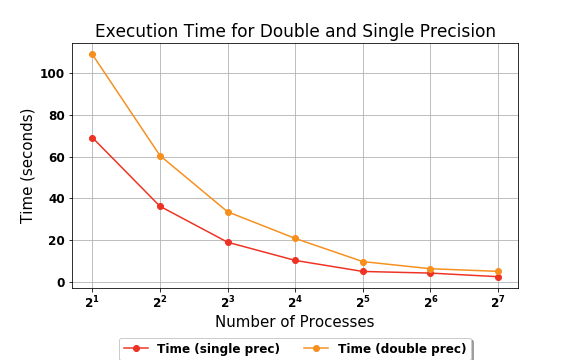
\includegraphics[width=1.\linewidth]{scaling_strong_log2.png}
		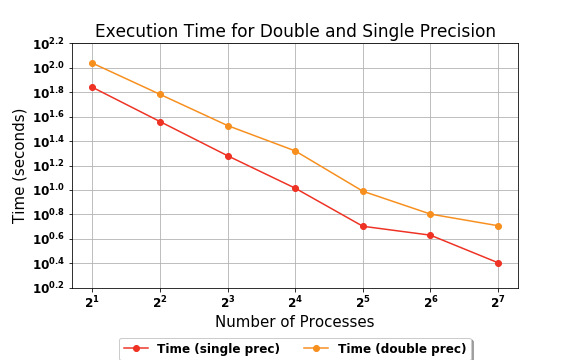
\includegraphics[width=1.\linewidth]{scaling_strong_log2log10.png}
		\caption{Strong scaling of execution time.}
		\label{fig:strong_scaling}
	\end{minipage}%
	\begin{minipage}{.5\linewidth}
		\centering
		%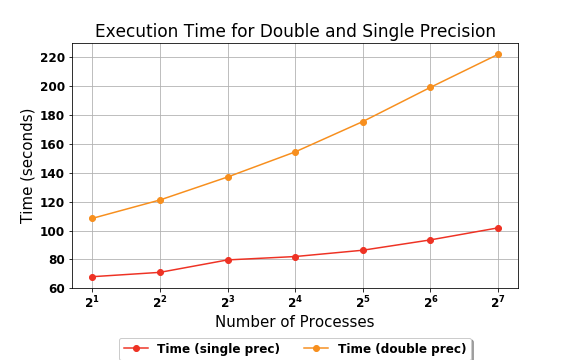
\includegraphics[width=1.\linewidth]{scaling_weak_log2.png}
		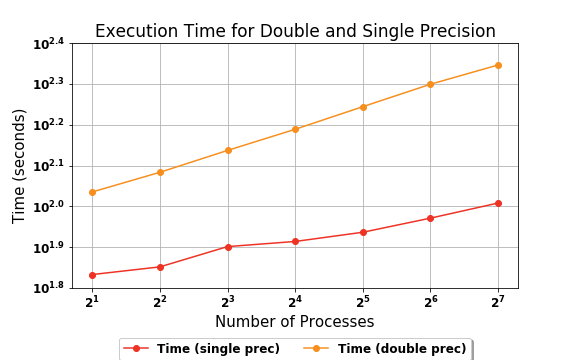
\includegraphics[width=1.\linewidth]{scaling_weak_log2log10.png}
		\caption{Weak scaling of execution time.}
		\label{fig:weak_scaling}
	\end{minipage}
\end{figure}

%---------------------------------------------------------------------------------

\subsection{Scalability Limitations}
\label{sec:scalability_limitations}
The limit on the maximum MPI message size prevented larger problem sizes being tested for the Intel Quantum Simulator. This limited the number of double precision states per process to be approximately $2^{27}$. Thus the simulator could not be tested up to the maximum available memory on a node.

To address this issue, the simulator was rebuilt using BigMPI instead of the standard MPI. However, the same problem persisted and BigMPI was later deprecated from being used with the simulator, reverting to standard MPI. As an alternative approach, Intel proposed running experiments on larger allocations on bigger European clusters, which would allow experiments using larger numbers of qubits, despite the memory on each node still being severely underutilised. To pursue this line of action, ICHEC plans on applying for a PRACE project to get the access to a larger HPC facility.

It is also noted that Intel advised that experiments with greater than two processes per node do not perform as well as for one or two processes. Thus, using many processes to fill a node's memory without exceeding the maximum MPI message size was deemed not to be a valid workaround.

%---------------------------------------------------------------------------------
%---------------------------------------------------------------------------------
\newpage
\section{Discussions and Summary}
\label{sec:discussion_and_summary}
Beginning with an outline of our proposed algorithmic approach in Section~\ref{sec:abstraction_of_disco_algorithms}, we discussed the steps required to realise the DisCo models for closest vector and sentence similarity from an implementation independent approach. The use of pre-computation allows us to effectively prepare our data into a format that may be represented in a quantum state. The pre-computed data may then be encoded into a quantum state using a viable method. Following this, we may directly use the closest vector, or sentence similarity algorithms as discussed by 
Zeng and Coecke~\cite{Zeng_Coecke_2016}.

We proceed to mention issues encountered with the state creation approach as proposed in the original work, where the use of QRAM models in quantum algorithm design presents challenges to small-scale count quantum computer systems and simulators with limited number of qubits. Workarounds for this were introduced, following the encoding approach of Trugenburger~\cite{Trugenberger_2001}, with the use of Hamming distance methods being effective to determine quantum state distance measures. 

An outline of the software architecture is proposed, wherein we make use of a two-tiered approach to perform pre-computation (implemented using Python) and subsequent encoding and evaluation (implemented using C++). Intel qHiPSTER is used within this latter layer to realise the quantum computing aspects of the described algorithms.

Our proposed testing and evaluation methodology is presented, and forms an outline for our design decisions. We aim for a granular procedure, wherein testing and evaluation follows a \emph{unit-integration-regression-acceptance} layout.

%Methodologies for testing and evaluating the implementation are outlined as well as a means to seamlessly apply continuous integration of these tests. This will allow for easy collection of additional performance metrics. We define the acceptance metrics for the implementation's results so that they can be validated.

The system requirements and software dependencies for the Intel Quantum Simulator are detailed. The simulator was observed to scale well for both weak and strong scaling. However, the limitations of the scaling for larger problem sizes are noted. A limited proposed workaround and the expected drawbacks are described; using a large node allocation on a bigger HPC cluster.

The next steps of this project involve implementing the algorithms and methods described in this report. After these algorithms have been implemented and their results are validated, we must integrate the different algorithms into a single software solution -- firstly, combining components of the Python and C++ implementations into modules, and following this integrating the Python and C++ modules to form one seamless application as illustrated in Figure~\ref{fig:qnlp_controlflow}. The results must be validated for the different corpora, which may require further refinement of the implementation. These steps will form the majority of the remaining work.

Furthermore, if time permits, different approaches to some of the above algorithms will be explored in greater detail. These algorithms involve an alternative to the DisCo model outlined in Appendix~\ref{app:loco_algo}, a Durr-Hoyer optimization of the Hamming distance approach in Appendix~\ref{app:hamming_dh}, and finally a state-rotation method for use with measurement-based state determination in Appendix \ref{app:ry_phase}.

%---------------------------------------------------------------------------------
%---------------------------------------------------------------------------------
\newpage
\begin{appendices}

\end{appendices}




%---------------------------------------------------------------------------------
\newpage
%---------------------------------------------------------------------------------
%---------------------------------------------------------------------------------
%\bibliographystyle{plain}
\bibliographystyle{unsrt}
\bibliography{Bibliography.bib}

\end{document}
